\documentclass[12pt,convert={false}]{standalone}
\usepackage[dvipsnames]{xcolor}
\usepackage{tikz}
\usetikzlibrary{shapes,arrows,positioning,calc,patterns,arrows.meta, bending, graphs, shadings,quotes,intersections}
\usetikzlibrary{external}
%\tikzexternalize[prefix=tikz/]
\usepackage{pgfplots}
\pgfplotsset{compat=1.16}
\usepgfplotslibrary{fillbetween}
\begin{document}
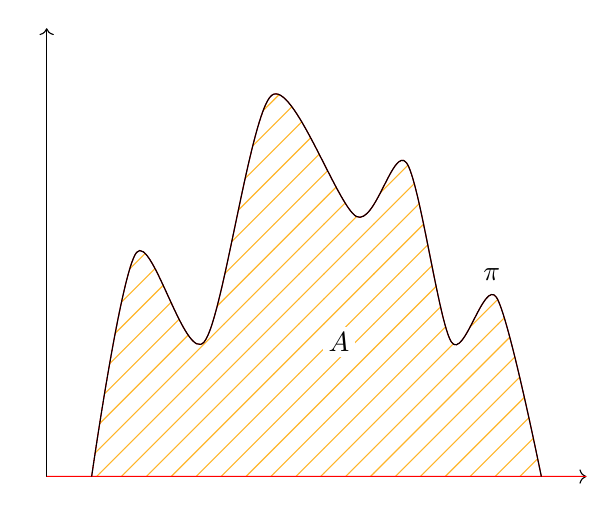
\begin{tikzpicture}
\pgfdeclarepatternformonly{ildiocane}%
   {\pgfqpoint{-1pt}{-1pt}}%
   {\pgfqpoint{10pt}{10pt}}%
   {\pgfqpoint{9pt}{9pt}}%
   {
     \pgfsetlinewidth{0.4pt}
     \pgfpathmoveto{\pgfqpoint{0pt}{0pt}}
     \pgfpathlineto{\pgfqpoint{9.1pt}{9.1pt}}
     \pgfusepath{stroke}
    }

\begin{axis}[
                xlabel=\empty,
                ticks=none,
                x axis line style={->,opacity=100},
                ylabel=\empty,
                xmin=0, xmax=1200,
                ymin=0, ymax=100,
                axis y line=left,
                y axis line style={->,opacity=100},
                axis x line*=bottom
                        ]
\addplot[smooth,name path=A] coordinates {
(100,0)
(200,50)
(350,30)
(500,85)
(689,58)
(800,70)
(900,30)
(1000,40)
(1100,0)
};
\path[name path=B] (axis cs:\pgfkeysvalueof{/pgfplots/xmin},0) -- (axis cs:\pgfkeysvalueof{/pgfplots/xmax},0);

    \addplot+[draw,pattern=ildiocane,pattern color=Dandelion]
    fill between[
        of=A and B,
        soft clip={domain=0:1},
    ];
 \node[align=left] at (990,45) {$\pi$};
 \node[fill=white,inner sep=2pt] at (650,30) {$A$};
\end{axis}
\end{tikzpicture}
\end{document}